Aqui vamos a detallar los resultados de las consultas que se realizaron en la base de datos, con el fin de obtener información relevante para la toma de decisiones. Cabe mencionar que las consultas se realizaron en PostgreSQL, y se utilizaron las tablas y vistas creadas en el esquema lógico de la base de datos. A continuación, se presentan las consultas realizadas y el analisis de los resultados obtenidos:
\begin{itemize}
    \item \textbf{Consulta 1:} \textbf{Entrenadores y Atletas, que compartan el apellido y que se encuentren participando en la misma disciplina.
Deberan ordenar la información a partir del apellido paterno.}\vspace{.3cm}
    \item \textbf{Consulta 2:} \section*{Consulta 2: Cantidad de asistentes y ganancias por disciplina y localidad}

\subsection*{Descripción}
Esta consulta calcula cuántas personas asistieron y cuánto dinero se ganó en cada disciplina y localidad. Es útil para evaluar el éxito financiero y la popularidad de los eventos en distintas áreas.

\textbf{SQL}

\begin{verbatim}
SELECT 
    d.NombreDisciplina,
    l.NombreLocalidad,
    SUM(e.Precio) AS GananciasTotales,
    COUNT(ce.IDCliente) AS CantidadAsistentes
FROM 
    Evento e
JOIN 
    Disciplina d ON e.IDDisciplina = d.IDDisciplina
JOIN 
    Localidad l ON e.NombreLocalidad = l.NombreLocalidad AND e.IDDisciplina = l.IDDisciplina
JOIN 
    CompraEntrada ce ON e.IDEvento = ce.IDEvento
GROUP BY 
    d.NombreDisciplina, l.NombreLocalidad
ORDER BY 
    CantidadAsistentes DESC;
\end{verbatim}

\begin{center}
    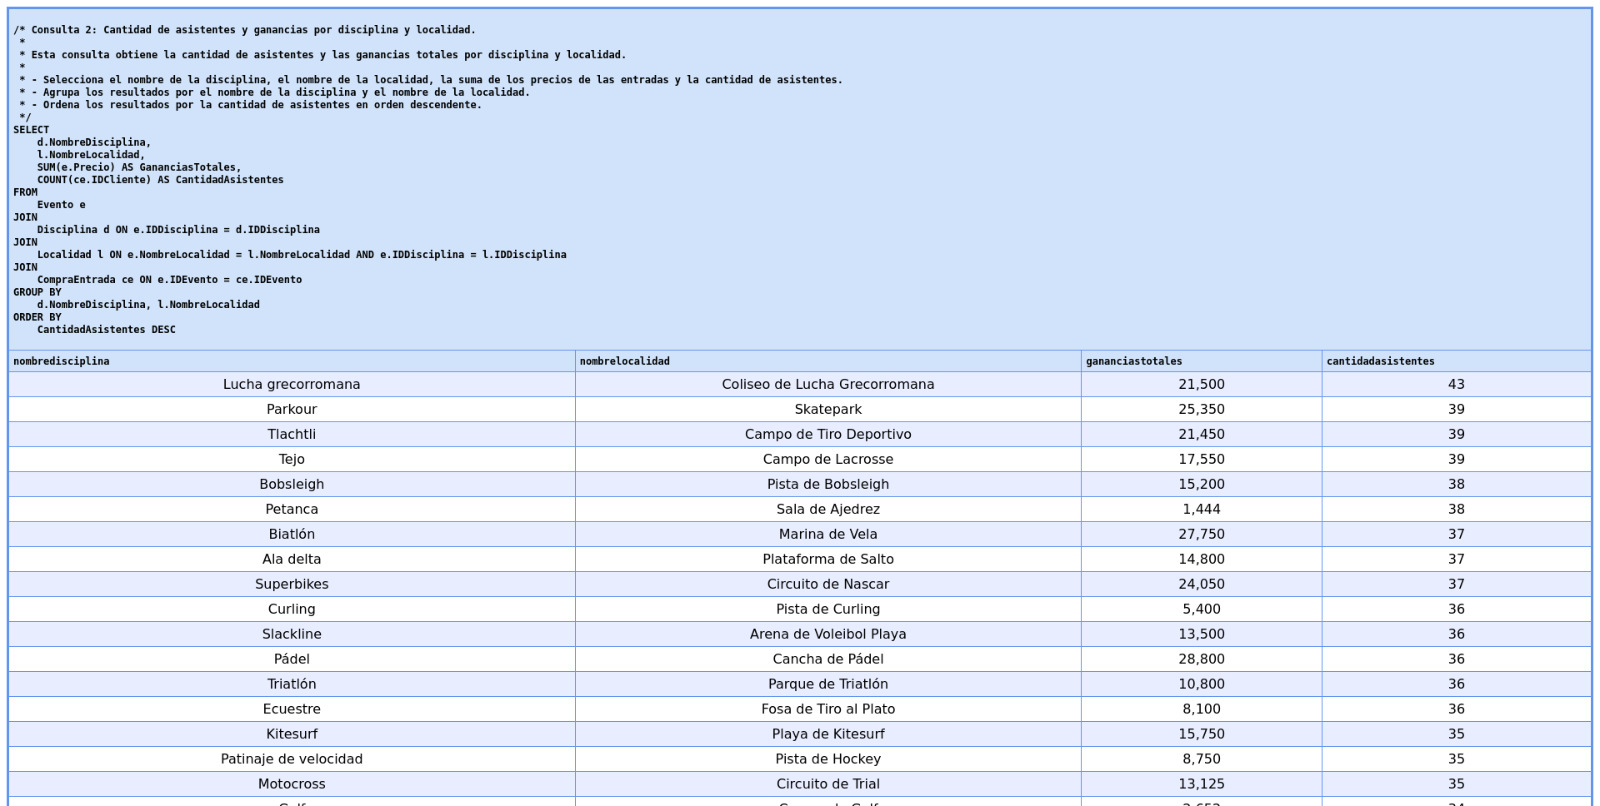
\includegraphics[width=16.5cm]{../resources/Chapters/Consultas/Imagenes/Consulta2.jpeg} 
    
   Consulta 2. Cantidad de asistentes y ganancias por disciplina y localidad. 
\end{center}

\textbf{Desglose de la consulta}

\begin{itemize}
   \item \textbf{Selección de columnas (\texttt{SELECT})}:
   \begin{itemize}
       \item Se seleccionan las siguientes columnas:
       \begin{itemize}
           \item \texttt{d.NombreDisciplina}: Nombre de la disciplina.
           \item \texttt{l.NombreLocalidad}: Nombre de la localidad.
           \item \texttt{SUM(e.Precio)}: Suma de los precios de las entradas, denominada \texttt{GananciasTotales}.
           \item \texttt{COUNT(ce.IDCliente)}: Cuenta la cantidad de asistentes, denominada \texttt{CantidadAsistentes}.
       \end{itemize}
   \end{itemize}
   
   \item \textbf{Tablas involucradas (\texttt{FROM} y \texttt{JOIN})}:
   \begin{itemize}
       \item La consulta utiliza cuatro tablas:
       \begin{itemize}
           \item \texttt{Evento (e)}: Contiene la información de los eventos.
           \item \texttt{Disciplina (d)}: Contiene la información de las disciplinas.
           \item \texttt{Localidad (l)}: Contiene la información de las localidades.
           \item \texttt{CompraEntrada (ce)}: Contiene la información de las entradas compradas.
       \end{itemize}
       \item Se realizan \texttt{JOINs} entre las tablas para relacionar los eventos con las disciplinas, localidades y entradas compradas.
   \end{itemize}
   
   \item \textbf{Agrupación de resultados (\texttt{GROUP BY})}:
   \begin{itemize}
       \item Para calcular la cantidad de asistentes y las ganancias por disciplina y localidad, se agrupan los datos según las columnas:
       \begin{itemize}
           \item \texttt{d.NombreDisciplina}, \texttt{l.NombreLocalidad}.
       \end{itemize}
       \item Esto garantiza que se genere un registro único por cada combinación de disciplina y localidad.
   \end{itemize}
   
   \item \textbf{Ordenamiento de resultados (\texttt{ORDER BY})}:
   \begin{itemize}
       \item Los resultados se ordenan por la columna \texttt{CantidadAsistentes} en orden descendente (\texttt{DESC}), de modo que las combinaciones de disciplina y localidad con más asistentes aparezcan primero.
   \end{itemize}
\end{itemize}

\textbf{Análisis detallado}

\begin{enumerate}
   \item \textbf{Relación entre tablas:}
   \begin{itemize}
       \item La consulta asume que existe una relación directa entre las tablas \texttt{Evento}, \texttt{Disciplina}, \texttt{Localidad} y \texttt{CompraEntrada} a través de las claves foráneas.
       \item Esto implica que:
       \begin{itemize}
           \item Cada evento está asociado con una disciplina y una localidad.
           \item Cada entrada comprada está asociada con un evento.
       \end{itemize}
   \end{itemize}
   
   \item \textbf{Uso de funciones agregadas \texttt{SUM} y \texttt{COUNT}:}
   \begin{itemize}
       \item La función \texttt{SUM(e.Precio)} calcula las ganancias totales generadas por las entradas vendidas para cada combinación de disciplina y localidad.
       \item La función \texttt{COUNT(ce.IDCliente)} cuenta el número de asistentes para cada combinación de disciplina y localidad.
   \end{itemize}
   
   \item \textbf{Agrupación por disciplina y localidad:}
   \begin{itemize}
       \item El uso de \texttt{GROUP BY} permite agrupar los registros por disciplina y localidad, asegurando que las ganancias y la cantidad de asistentes se calculen correctamente para cada combinación.
   \end{itemize}
   
   \item \textbf{Ordenamiento:}
   \begin{itemize}
       \item El orden descendente por \texttt{CantidadAsistentes} facilita la identificación de las combinaciones de disciplina y localidad con mayor número de asistentes.
   \end{itemize}
\end{enumerate}

\textbf{Consideraciones}

\begin{itemize}
   \item \textbf{Empates en la cantidad de asistentes:}
   \begin{itemize}
       \item Si varias combinaciones de disciplina y localidad tienen la misma cantidad de asistentes, el orden relativo entre ellas no está definido. Para resolver esto, se podría agregar un criterio adicional en el \texttt{ORDER BY}, como las ganancias totales.
   \end{itemize}
\end{itemize}

    \item  \textbf{Consulta 3:} \textbf{Atletas que hayan participado en más de 1 disciplina.}\vspace{.3cm}
    \item \textbf{Consulta 4:} 
Cómo modificarías el diagrama de la figura a) para representar las siguientes restricciones:\\
Un alumno no puede tomar clase en más de una materia con el mismo profesor. Una materia no puede ser
impartida por más de un profesor.

No es necesario realizar alguna modificación, pues la cardinalidad uno a uno que tiene el diagrama implica que un alumno no puede estar relacionado con el mismo profesor en más de una materia, y del mismo modo una materia no puede ser impartida por más de un profesor en la relación, por lo que el diagrama ya cumple con ambas restricciones.

    \item \textbf{Consulta 5:} \begin{center}
    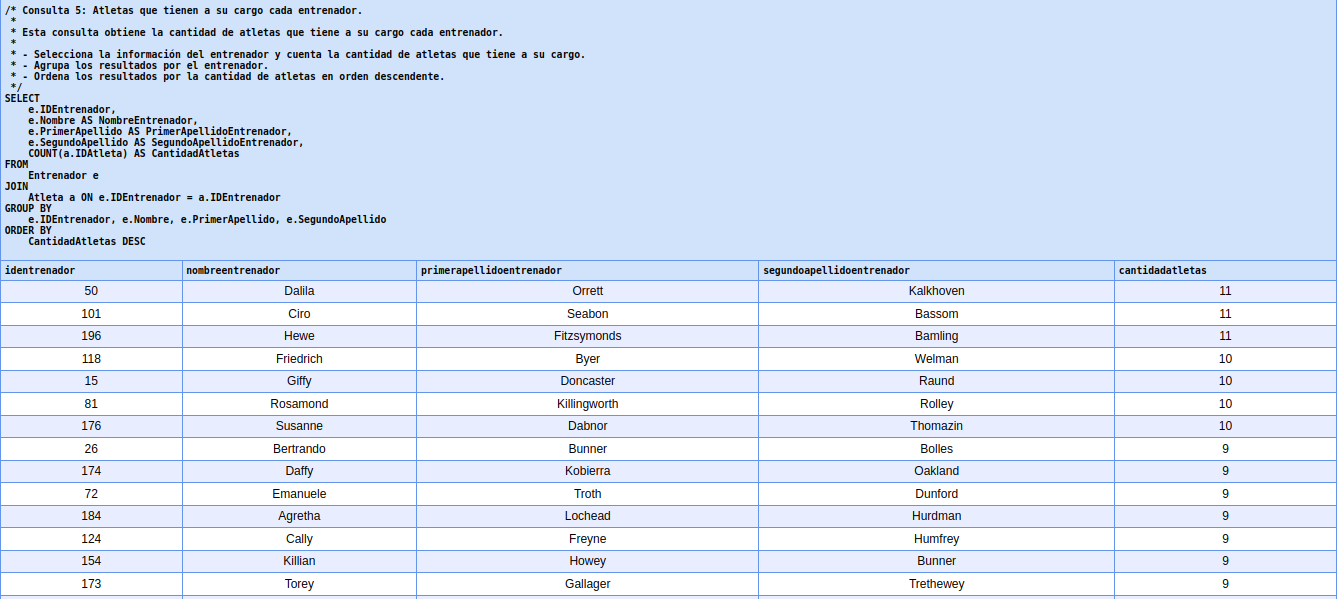
\includegraphics[width=16.5cm]{../resources/Chapters/Consultas/Imagenes/Consulta5.png} 
    
   Consulta 5. Atletas que tienen a su cargo cada entrenador. 
\end{center}

\textbf{Propósito de la consulta}

La consulta tiene como objetivo obtener un listado de entrenadores junto con la cantidad de atletas que tienen a su cargo. Esto es útil para entender la distribución de atletas entre los entrenadores y detectar posibles desequilibrios en la asignación de recursos.

\textbf{Desglose de la consulta}

\begin{itemize}
   \item \textbf{Selección de columnas (\texttt{SELECT})}:
   \begin{itemize}
       \item Se seleccionan las siguientes columnas del entrenador:
       \begin{itemize}
           \item \texttt{e.IDEntrenador}: Identificador único del entrenador.
           \item \texttt{e.Nombre}: Nombre del entrenador.
           \item \texttt{e.PrimerApellido}: Primer apellido del entrenador.
           \item \texttt{e.SegundoApellido}: Segundo apellido del entrenador.
       \end{itemize}
       \item Se utiliza la función agregada \texttt{COUNT(a.IDAtleta)} para contar cuántos atletas están asociados con cada entrenador. Esta columna se denomina \texttt{CantidadAtletas}.
   \end{itemize}
   
   \item \textbf{Tablas involucradas (\texttt{FROM} y \texttt{JOIN})}:
   \begin{itemize}
       \item La consulta utiliza dos tablas:
       \begin{itemize}
           \item \texttt{Entrenador (e)}: Contiene la información de los entrenadores.
           \item \texttt{Atleta (a)}: Contiene la información de los atletas.
       \end{itemize}
       \item Se realiza un \texttt{JOIN} entre ambas tablas utilizando la relación \texttt{e.IDEntrenador = a.IDEntrenador}. Esto asegura que solo se consideren los atletas que están asignados a un entrenador.
   \end{itemize}
   
   \item \textbf{Agrupación de resultados (\texttt{GROUP BY})}:
   \begin{itemize}
       \item Para calcular la cantidad de atletas por entrenador, se agrupan los datos según las columnas únicas del entrenador:
       \begin{itemize}
           \item \texttt{e.IDEntrenador}, \texttt{e.Nombre}, \texttt{e.PrimerApellido}, \texttt{e.SegundoApellido}.
       \end{itemize}
       \item Esto garantiza que se genere un registro único por cada entrenador.
   \end{itemize}
   
   \item \textbf{Ordenamiento de resultados (\texttt{ORDER BY})}:
   \begin{itemize}
       \item Los resultados se ordenan por la columna \texttt{CantidadAtletas} en orden descendente (\texttt{DESC}), de modo que los entrenadores con más atletas aparezcan primero.
   \end{itemize}
\end{itemize}

\textbf{Análisis detallado}

\begin{enumerate}
   \item \textbf{Relación entre tablas:}
   \begin{itemize}
       \item La consulta asume que existe una relación directa entre las tablas \texttt{Entrenador} y \texttt{Atleta} a través de la clave foránea \texttt{a.IDEntrenador}, que apunta a \texttt{e.IDEntrenador}.
       \item Esto implica que:
       \begin{itemize}
           \item Cada atleta tiene asignado exactamente un entrenador.
           \item Un entrenador puede tener asignados uno o más atletas.
       \end{itemize}
   \end{itemize}
   
   \item \textbf{Uso de la función agregada \texttt{COUNT}:}
   \begin{itemize}
       \item La función \texttt{COUNT(a.IDAtleta)} cuenta el número de registros en la tabla \texttt{Atleta} que están relacionados con cada entrenador.
       \item Si un entrenador no tiene atletas asignados, no aparecerá en los resultados porque el \texttt{JOIN} elimina las filas sin coincidencias.
   \end{itemize}
   
   \item \textbf{Agrupación por entrenador:}
   \begin{itemize}
       \item El uso de \texttt{GROUP BY} permite agrupar los registros por entrenador, asegurando que la cantidad de atletas se calcule correctamente para cada uno.
   \end{itemize}
   
   \item \textbf{Ordenamiento:}
   \begin{itemize}
       \item El orden descendente por \texttt{CantidadAtletas} facilita la identificación de los entrenadores con mayor carga de trabajo.
   \end{itemize}
\end{enumerate}

\textbf{Consideraciones}

\begin{itemize}
   
   \item \textbf{Empates en la cantidad de atletas:}
   \begin{itemize}
       \item Si varios entrenadores tienen la misma cantidad de atletas, el orden relativo entre ellos no está definido. Para resolver esto, se podría agregar un criterio adicional en el \texttt{ORDER BY}, como el nombre del entrenador.
   \end{itemize}
\end{itemize}

    \item \textbf{Consulta 6:} \begin{center}
    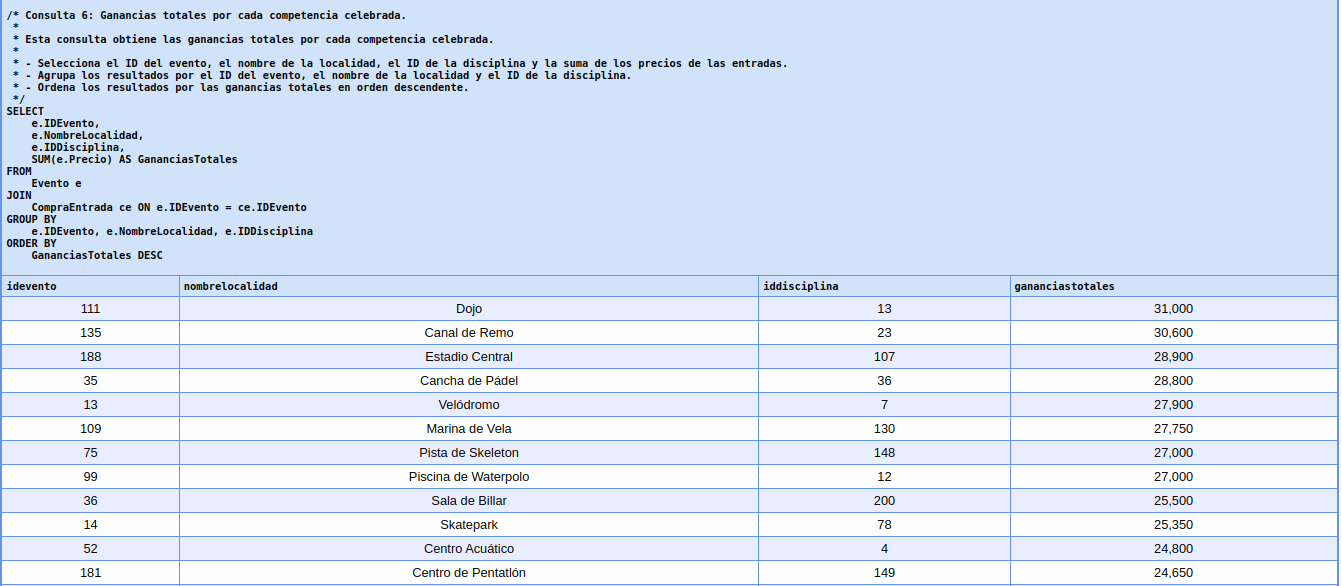
\includegraphics[width=16.5cm]{resources/Chapters/Consultas/Imagenes/Consulta6.png} 
    
   Consulta 6. Ganancias totales por cada competencia celebrada.
\end{center}

\textbf{Propósito de la consulta}

La consulta tiene como objetivo calcular las ganancias totales generadas por la venta de entradas para cada competencia celebrada. Esto permite identificar qué eventos fueron más rentables y en qué localidades o disciplinas se generaron mayores ingresos.

\textbf{Desglose de la consulta}

\begin{itemize}
   \item \textbf{Selección de columnas (\texttt{SELECT}):}
   \begin{itemize}
       \item \texttt{e.IDEvento}: Identificador único del evento, que permite distinguir cada competencia.
       \item \texttt{e.NombreLocalidad}: Nombre de la localidad donde se celebró el evento.
       \item \texttt{e.IDDisciplina}: Identificador de la disciplina deportiva asociada al evento.
       \item \texttt{SUM(e.Precio) AS GananciasTotales}: Calcula la suma total de los precios de las entradas vendidas para cada evento, representando las ganancias totales.
   \end{itemize}

   \item \textbf{Tablas involucradas (\texttt{FROM} y \texttt{JOIN}):}
   \begin{itemize}
       \item \texttt{Evento (e)}: Contiene información sobre los eventos celebrados, como su identificador, localidad y disciplina.
       \item \texttt{CompraEntrada (ce)}: Registra las compras de entradas realizadas para los eventos.
       \item \textbf{Unión (\texttt{JOIN})}: Se realiza un \texttt{JOIN} entre ambas tablas utilizando la relación \texttt{e.IDEvento = ce.IDEvento}, asegurando que solo se consideren las entradas compradas para eventos específicos.
   \end{itemize}

   \item \textbf{Agrupación de resultados (\texttt{GROUP BY}):}
   \begin{itemize}
       \item La agrupación se realiza por las siguientes columnas:
       \begin{itemize}
           \item \texttt{e.IDEvento}: Para agrupar las ganancias por cada evento específico.
           \item \texttt{e.NombreLocalidad}: Para asociar las ganancias con la localidad donde se celebró el evento.
           \item \texttt{e.IDDisciplina}: Para distinguir las ganancias según la disciplina deportiva del evento.
       \end{itemize}
       \item Esto permite calcular la suma de los precios de las entradas (\texttt{SUM(e.Precio)}) de manera independiente para cada combinación de evento, localidad y disciplina.
   \end{itemize}

   \item \textbf{Ordenamiento de resultados (\texttt{ORDER BY}):}
   \begin{itemize}
       \item Los resultados se ordenan por la columna \texttt{GananciasTotales} en orden descendente (\texttt{DESC}), de modo que los eventos con mayores ganancias aparezcan primero.
   \end{itemize}
\end{itemize}

\textbf{Análisis detallado}

\begin{itemize}
   \item \textbf{Relación entre tablas:}
   \begin{itemize}
       \item La consulta asume que existe una relación directa entre las tablas \texttt{Evento} y \texttt{CompraEntrada} mediante la clave foránea \texttt{ce.IDEvento}, que apunta a \texttt{e.IDEvento}.
       \item Esto implica que cada entrada comprada está asociada a un único evento y que un evento puede tener múltiples entradas compradas.
   \end{itemize}

   \item \textbf{Uso de la función agregada \texttt{SUM}:}
   \begin{itemize}
       \item La función \texttt{SUM(e.Precio)} calcula la suma total de los precios de las entradas vendidas para cada evento.
       \item Se supone que el campo \texttt{Precio} en la tabla \texttt{Evento} representa el precio de una entrada individual y que este valor se multiplica implícitamente por el número de entradas compradas en la tabla \texttt{CompraEntrada}.
   \end{itemize}

   \item \textbf{Agrupación por columnas clave:}
   \begin{itemize}
       \item La agrupación por \texttt{e.IDEvento}, \texttt{e.NombreLocalidad} y \texttt{e.IDDisciplina} asegura que las ganancias se calculen de manera específica para cada combinación de:
       \begin{itemize}
           \item Evento único (\texttt{e.IDEvento}).
           \item Localidad donde se celebró el evento (\texttt{e.NombreLocalidad}).
           \item Disciplina deportiva asociada al evento (\texttt{e.IDDisciplina}).
       \end{itemize}
   \end{itemize}

   \item \textbf{Ordenamiento por ganancias:}
   \begin{itemize}
       \item Ordenar los resultados por \texttt{GananciasTotales} en orden descendente permite identificar fácilmente los eventos más rentables.
   \end{itemize}
\end{itemize}

\textbf{Posibles escenarios y consideraciones}

\begin{itemize}
   \item \textbf{Eventos sin entradas vendidas:}
   \begin{itemize}
       \item Si un evento no tiene entradas vendidas, no aparecerá en los resultados debido al \texttt{JOIN}. Esto significa que solo se mostrarán eventos con al menos una entrada comprada.
   \end{itemize}

   \item \textbf{Localidades y disciplinas:}
   \begin{itemize}
       \item Los resultados permiten identificar no solo los eventos más rentables, sino también qué localidades y disciplinas deportivas generan mayores ingresos.
   \end{itemize}

   \item \textbf{Empates en las ganancias:}
   \begin{itemize}
       \item Si dos o más eventos tienen las mismas ganancias totales, el orden relativo entre ellos no está definido. Esto no afecta el propósito principal de la consulta, pero podría ser relevante en algunos análisis.
   \end{itemize}
\end{itemize}

La consulta está diseñada para calcular las ganancias totales generadas por cada evento, agrupadas por localidad y disciplina. Es útil para identificar eventos, localidades y disciplinas con mayor rentabilidad, lo que puede ser clave para la planificación de futuros eventos deportivos.

    \item \textbf{Consulta 7:} \textbf{El número de medallas de plata ganadas por Japón.}\vspace{.3cm}

Para resolver esta consulta, primero identificamos la necesidad de acceder a la información sobre la nacionalidad de los atletas y el tipo de medalla ganada. Por lo tanto, estructuramos nuestra consulta de la siguiente manera: \vspace{.3cm}

\begin{lstlisting}
    SELECT 
    COUNT(*) AS medallas_plata
FROM 
    Medalla m
JOIN 
    Atleta a ON m.IDAtleta = a.IDAtleta
WHERE 
    a.Nacionalidad = 'Japonesa' AND m.TipoMedalla = 'Plata';
\end{lstlisting}

 \vspace{.3cm}

Primero, seleccionamos la tabla Medalla y la aliasamos como m. Luego, realizamos un (JOIN) con la tabla Atleta, aliasada como a, utilizando la columna IDAtleta que es común en ambas tablas. Por lo cual dado este join, se nos permite acceder a la información de los atletas que han ganado medallas. \\

Despues, seleccionamos la tabla Medalla para contar cuántas medallas de plata ha ganado Japón. Utilizando la función COUNT(*) para contar todas las filas que cumplen con las condiciones especificadas en el WHERE, es decir, aquellas donde la nacionalidad del atleta es 'Japonesa' y el tipo de medalla es 'Plata'. \vspace{.3cm}

El resultado es un único valor que representa el total de medallas de plata ganadas por Japón ya que es lo unico que se nos pide \textit{(el número de medallas de plata ganadas por Japón)}. \vspace{.3cm}

\textbf{Resultado:}
\begin{center}
    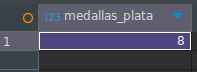
\includegraphics[width=10cm]{resources/resultados/r7.png}
\end{center}   

Nota: Para obtener este resultado, se añadieron manualmente registros en la tabla Medalla para asegurar que Japón tenga medallas de plata registradas. \vspace{.3cm}
    \item \textbf{Consulta 8:} \textbf{El número de medallas de bronce ganadas por España.}\vspace{.3cm}

Ahora similar al caso anterior realizamos lo analogo pero para España: \vspace{.3cm}

\begin{lstlisting}
    SELECT 
    COUNT(*) AS medallas_bronce
FROM 
    Medalla m
JOIN 
    Atleta a ON m.IDAtleta = a.IDAtleta
WHERE 
    a.NombrePais = 'Espana' AND m.TipoMedalla = 'Bronce';
\end{lstlisting}

\vspace{.3cm}

En esta consulta, seleccionamos la tabla Medalla para contar el número de medallas de bronce ganadas por España. Utilizamos la función COUNT(*) para contar todas las filas que cumplen con las condiciones especificadas en el WHERE, es decir, aquellas donde el país es 'España' y el tipo de medalla es 'Bronce'. \vspace{.3cm}

El resultado es un solo valor que representa el número total de medallas de bronce ganadas por España \textit{(analogo al inciso anterior)}. \vspace{.3cm}

\textbf{Resultado:}
\begin{center}
    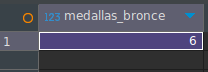
\includegraphics[width=10cm]{resources/resultados/r8.png}
\end{center}   

Nota: Para este resultado, tambien se añadieron manualmente tuplas en la tabla Medalla. \vspace{.3cm}
    \item \textbf{Consulta 9:} \textbf{La información de los atletas que ganaron medallas en la disciplina halterofilia.}\vspace{.3cm}

Para esta consulta, lo resolví de la siguiente manera: \vspace{.3cm}

\begin{lstlisting}
    SELECT 
    a.IDAtleta,
    a.Nombre,
    a.PrimerApellido,
    a.SegundoApellido,
    a.FechaNacimiento,
    a.Nacionalidad,
    a.Genero,
    m.TipoMedalla
FROM 
    Medalla m
JOIN 
    Atleta a ON m.IDAtleta = a.IDAtleta
JOIN 
    Disciplina d ON m.IDDisciplina = d.IDDisciplina
WHERE 
    d.NombreDisciplina = 'Halterofilia';
\end{lstlisting}

\textbf{Explicación:} \vspace{.3cm}

En esta consulta, seleccionamos la tabla `atleta` para obtener la información de los atletas que han ganado medallas en la disciplina de halterofilia. Utilizamos un `JOIN` con la tabla `medalla` para relacionar los atletas con las medallas que han ganado. Luego, filtramos los resultados para incluir solo aquellos donde la disciplina de la medalla es 'Halterofilia'. \vspace{.3cm}

El resultado es un conjunto de filas que representan a los atletas que han ganado medallas en la disciplina de halterofilia. \vspace{.3cm}

\textbf{Resultado:}
\begin{center}
    
\end{center}   

Nota: Para este resultado, se añadieron manualmente tuplas en la tabla `medalla` para asegurar que haya registros de medallas en la disciplina de halterofilia. \vspace{.3cm}
    \item \textbf{Consulta 10:} \begin{center}
	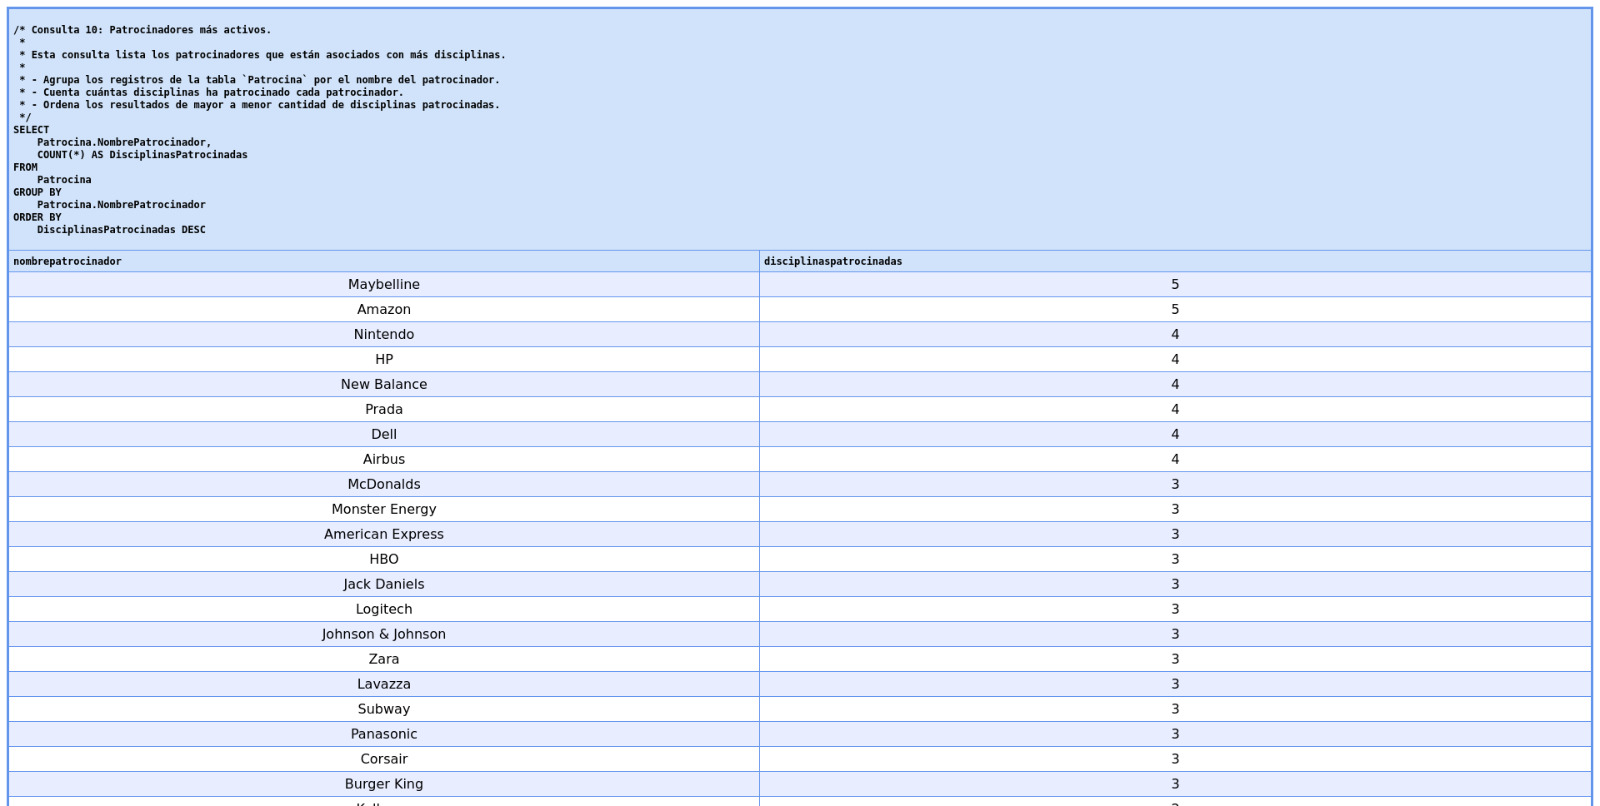
\includegraphics[width=16.5cm]{resources/Chapters/Consultas/Imagenes/Consulta10.jpg} 
	
	Consulta 10. Patrocinadores más activos. 
\end{center}

\textbf{Propósito de la consulta}

La consulta tiene como objetivo identificar a los patrocinadores más activos, es decir, aquellos que están asociados con la mayor cantidad de disciplinas patrocinadas. Los resultados se ordenan de mayor a menor según el número de disciplinas patrocinadas.

\textbf{Desglose de la consulta}

\begin{itemize} \item \textbf{Selección de columnas (\texttt{SELECT}):} \begin{itemize} \item \texttt{Patrocina.NombrePatrocinador}: Nombre del patrocinador, que identifica de forma única a cada entidad patrocinadora. \item \texttt{COUNT(*) AS DisciplinasPatrocinadas}: Cuenta el número total de disciplinas patrocinadas por cada patrocinador. \end{itemize}
	
	\item \textbf{Tabla involucrada (\texttt{FROM}):} \begin{itemize} \item \texttt{Patrocina}: Tabla que almacena la relación entre patrocinadores y disciplinas patrocinadas. \end{itemize}
	
	\item \textbf{Agrupación de resultados (\texttt{GROUP BY}):} \begin{itemize} \item \texttt{Patrocina.NombrePatrocinador}: Agrupa los registros por el nombre del patrocinador para calcular cuántas disciplinas ha patrocinado cada uno. \end{itemize}
	
	\item \textbf{Ordenamiento de resultados (\texttt{ORDER BY}):} \begin{itemize} \item Los resultados se ordenan por \texttt{DisciplinasPatrocinadas} en orden descendente (\texttt{DESC}), de modo que los patrocinadores más activos aparezcan primero. \end{itemize} \end{itemize}

\textbf{Análisis detallado}

\begin{itemize} \item \textbf{Relación entre patrocinadores y disciplinas:} \begin{itemize} \item La tabla \texttt{Patrocina} registra las asociaciones entre los patrocinadores y las disciplinas que apoyan, lo que permite calcular la cantidad de disciplinas patrocinadas por cada patrocinador. \end{itemize}
	
	\item \textbf{Uso de la función agregada \texttt{COUNT}:} \begin{itemize} \item \texttt{COUNT(*)} cuenta el número total de registros asociados con cada patrocinador, lo que representa el número de disciplinas que han patrocinado. \end{itemize}
	
	\item \textbf{Agrupación por patrocinador:} \begin{itemize} \item La agrupación por \texttt{Patrocina.NombrePatrocinador} asegura que el conteo de disciplinas patrocinadas sea específico para cada patrocinador. \end{itemize}
	
	\item \textbf{Ordenamiento por actividad:} \begin{itemize} \item Ordenar los resultados por \texttt{DisciplinasPatrocinadas} permite identificar fácilmente a los patrocinadores más activos. \end{itemize} \end{itemize}

\textbf{Posibles escenarios y consideraciones}

\begin{itemize} \item \textbf{Patrocinadores sin disciplinas asociadas:} \begin{itemize} \item Si un patrocinador no tiene disciplinas asociadas en la tabla \texttt{Patrocina}, no aparecerá en los resultados, ya que \texttt{COUNT(*)} excluye registros inexistentes. \end{itemize}
	
	\item \textbf{Empates en la actividad:} \begin{itemize} \item Si dos o más patrocinadores tienen la misma cantidad de disciplinas patrocinadas, el orden relativo entre ellos no está definido. \end{itemize}
	
	\item \textbf{Interpretación de los resultados:} \begin{itemize} \item La consulta solo refleja la cantidad de disciplinas patrocinadas, pero no considera otros factores como la inversión o la duración del patrocinio. \end{itemize} \end{itemize}

La consulta proporciona una lista clara de los patrocinadores más activos en términos de disciplinas apoyadas, lo que puede ser útil para evaluar la participación y el impacto de los patrocinadores en el evento.
    \item \textbf{Consulta 11:} \begin{center}
	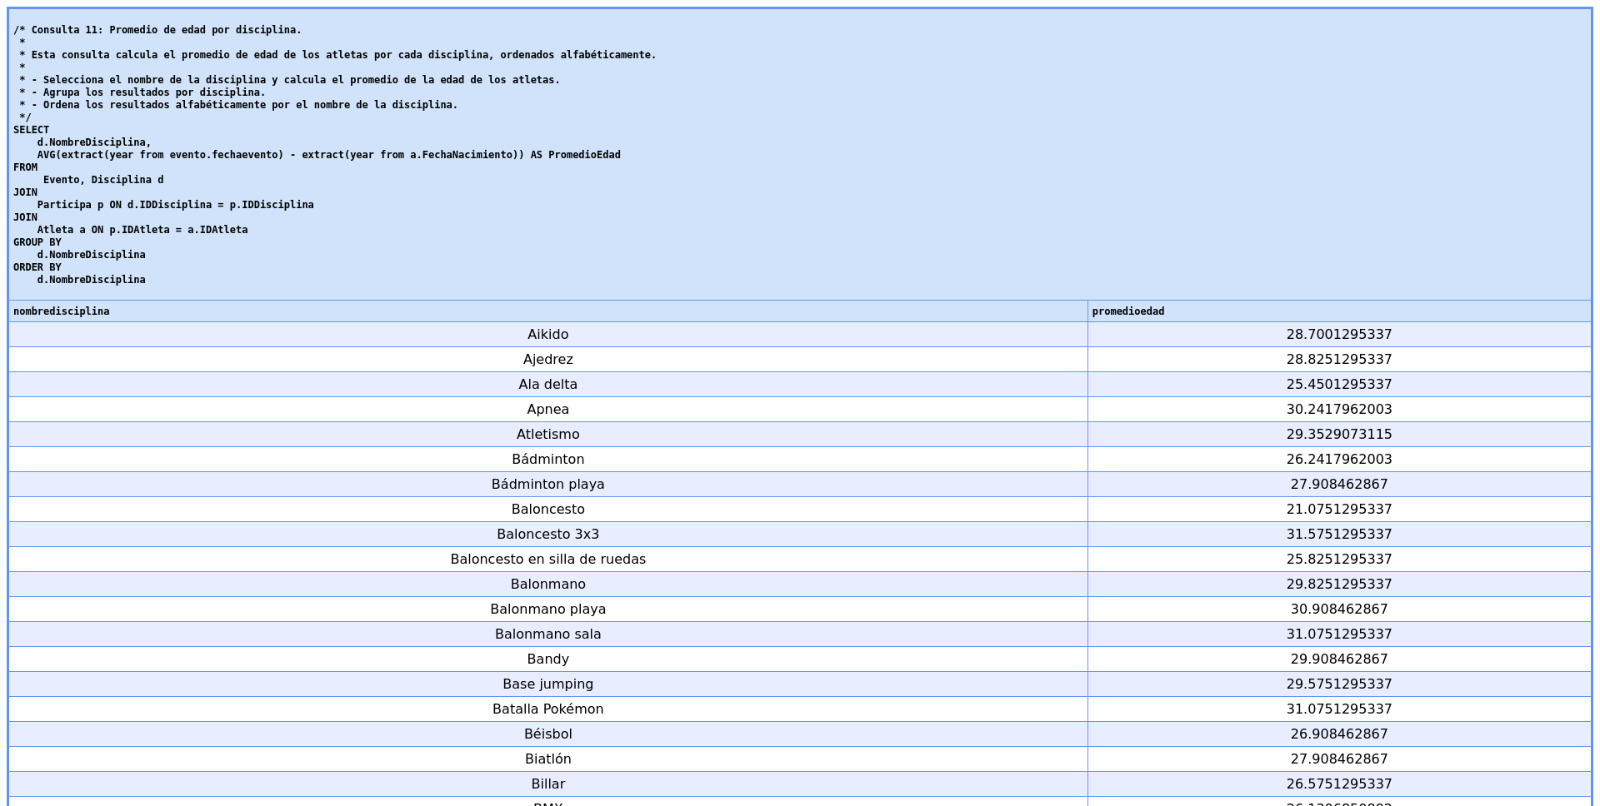
\includegraphics[width=16.5cm]{resources/Chapters/Consultas/Imagenes/Consulta11.jpg} 
	
	Consulta 11. Promedio de edad por disciplina.
\end{center}

\textbf{Propósito de la consulta}

La consulta tiene como objetivo calcular el promedio de edad de los atletas por cada disciplina deportiva. Los resultados están ordenados alfabéticamente por el nombre de la disciplina para facilitar su interpretación.

\textbf{Desglose de la consulta}

\begin{itemize} \item \textbf{Selección de columnas (\texttt{SELECT}):} \begin{itemize} \item \texttt{d.NombreDisciplina}: El nombre de la disciplina, que identifica de forma única cada deporte o actividad. \item \texttt{AVG(EXTRACT(YEAR FROM evento.FechaEvento) - EXTRACT(YEAR FROM a.FechaNacimiento)) AS PromedioEdad}: Calcula el promedio de la diferencia de años entre la fecha del evento y la fecha de nacimiento de los atletas, representando el promedio de edad para cada disciplina. \end{itemize}
	
	\item \textbf{Tablas involucradas (\texttt{FROM} y \texttt{JOIN}):} \begin{itemize} \item \texttt{Evento}: Tabla que contiene información sobre los eventos, incluida la fecha en que se llevaron a cabo. \item \texttt{Disciplina (d)}: Tabla que registra las disciplinas deportivas disponibles. \item \texttt{Participa (p)}: Relaciona a los atletas con las disciplinas en las que participan. \item \texttt{Atleta (a)}: Tabla que almacena información sobre los atletas, incluida su fecha de nacimiento. \item \textbf{Uniones (\texttt{JOIN})}: \begin{itemize} \item Se realiza un \texttt{JOIN} entre \texttt{Disciplina (d)} y \texttt{Participa (p)} usando la clave \texttt{d.IDDisciplina = p.IDDisciplina}. \item Posteriormente, se une \texttt{Atleta (a)} con \texttt{Participa (p)} usando \texttt{p.IDAtleta = a.IDAtleta}. \end{itemize} \end{itemize}
	
	\item \textbf{Agrupación de resultados (\texttt{GROUP BY}):} \begin{itemize} \item La agrupación se realiza por \texttt{d.NombreDisciplina}, lo que permite calcular el promedio de edad de los atletas de forma independiente para cada disciplina. \end{itemize}
	
	\item \textbf{Ordenamiento de resultados (\texttt{ORDER BY}):} \begin{itemize} \item Los resultados se ordenan alfabéticamente por el nombre de la disciplina (\texttt{d.NombreDisciplina}), facilitando su organización y lectura. \end{itemize} \end{itemize}

\textbf{Análisis detallado}

\begin{itemize} \item \textbf{Relación entre tablas:} \begin{itemize} \item La consulta utiliza varias tablas relacionadas: \begin{itemize} \item La tabla \texttt{Disciplina (d)} se conecta con \texttt{Participa (p)} para identificar las disciplinas en las que participan los atletas. \item La tabla \texttt{Atleta (a)} proporciona la información de la fecha de nacimiento de cada atleta, necesaria para calcular su edad. \end{itemize} \item La tabla \texttt{Evento} se utiliza para calcular la edad de los atletas en el año en que ocurrió el evento. \end{itemize}
	
	\item \textbf{Cálculo del promedio de edad:} \begin{itemize} \item La función \texttt{AVG()} calcula el promedio de la diferencia entre: \begin{itemize} \item El año del evento (\texttt{EXTRACT(YEAR FROM evento.FechaEvento)}). \item El año de nacimiento del atleta (\texttt{EXTRACT(YEAR FROM a.FechaNacimiento)}). \end{itemize} \item Esto representa el promedio de edad de los atletas para cada disciplina en el año del evento. \end{itemize}
	
	\item \textbf{Ordenamiento alfabético:} \begin{itemize} \item Ordenar los resultados por \texttt{d.NombreDisciplina} garantiza que las disciplinas estén organizadas de forma alfabética, mejorando la presentación de los datos. \end{itemize} \end{itemize}

\textbf{Posibles escenarios y consideraciones}

\begin{itemize} \item \textbf{Disciplinas sin participación:} \begin{itemize} \item Si una disciplina no tiene atletas registrados en \texttt{Participa}, no aparecerá en los resultados debido al uso de \texttt{JOIN}, lo que implica que solo se consideran disciplinas con participantes. \end{itemize}
	
	\item \textbf{Edad promedio en decimal:} \begin{itemize} \item Los resultados del promedio de edad pueden incluir decimales, lo que representa una aproximación más precisa. \end{itemize}
	
	\item \textbf{Datos de fechas:} \begin{itemize} \item Es importante que las fechas (\texttt{evento.FechaEvento} y \texttt{a.FechaNacimiento}) estén correctamente registradas para evitar errores en el cálculo de la edad. \end{itemize} \end{itemize}

La consulta está diseñada para calcular de manera eficiente el promedio de edad de los atletas por disciplina, proporcionando información valiosa para análisis demográficos y de participación en los eventos deportivos.
    \item \textbf{Consulta 12:} \begin{center}
    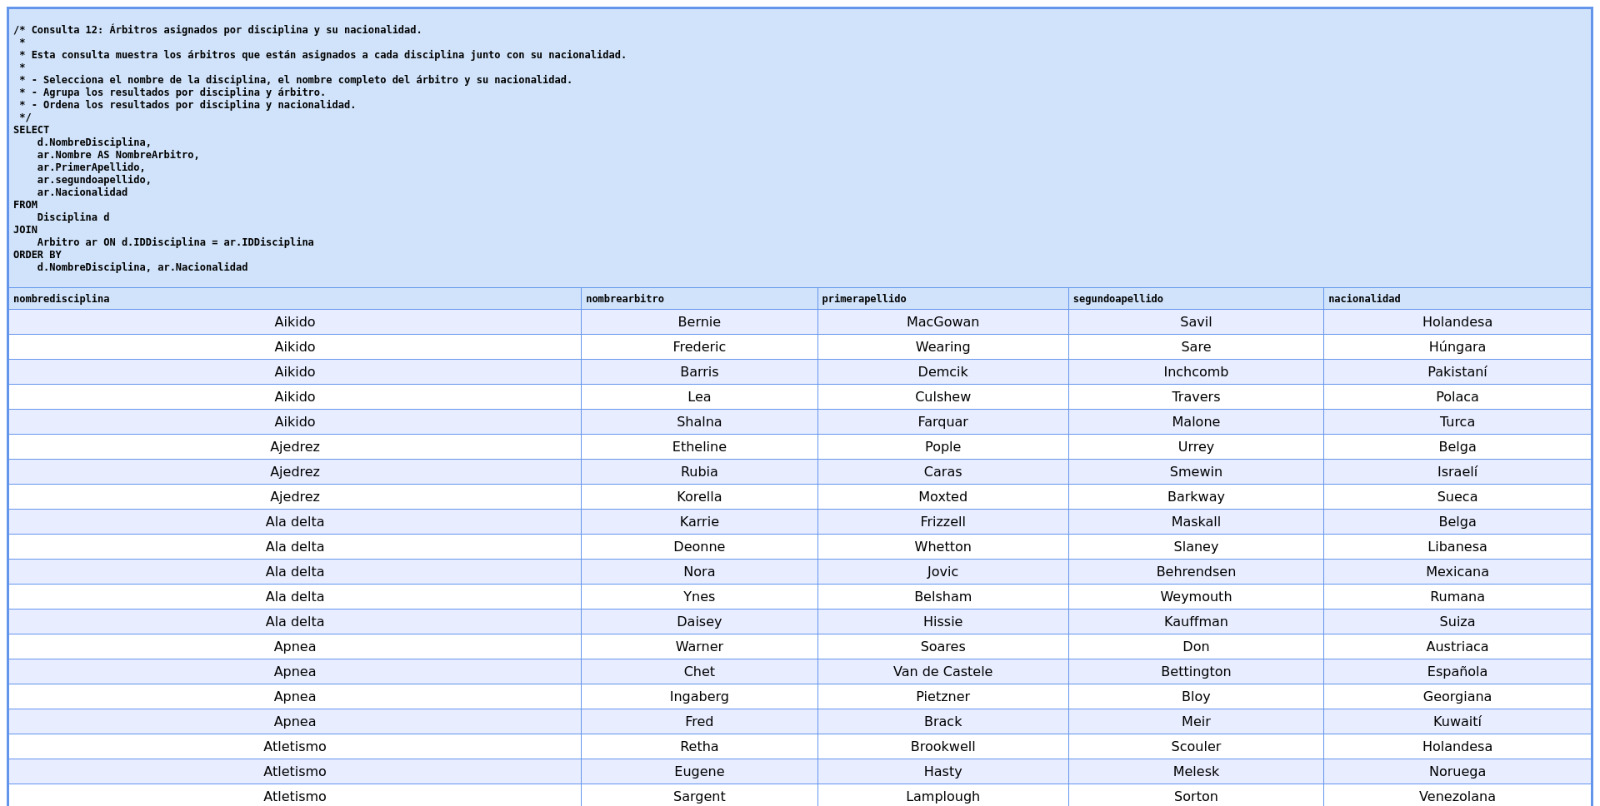
\includegraphics[width=16.5cm]{resources/Consulta12.jpeg} 
    
   Consulta 12. Árbitros asignados por disciplina y su nacionalidad.
\end{center}

\textbf{Propósito de la consulta}

El objetivo de esta consulta es obtener una lista de los árbitros asignados a cada disciplina, incluyendo su nacionalidad. Esto permite analizar la distribución de los árbitros entre las disciplinas y verificar la diversidad cultural representada en el equipo de árbitros.

\textbf{Desglose de la consulta}

\begin{itemize}
   \item \textbf{Selección de columnas (\texttt{SELECT})}:
   \begin{itemize}
       \item \texttt{d.NombreDisciplina}: Nombre de la disciplina deportiva.
       \item \texttt{ar.Nombre}: Nombre del árbitro.
       \item \texttt{ar.PrimerApellido} y \texttt{ar.SegundoApellido}: Apellidos del árbitro.
       \item \texttt{ar.Nacionalidad}: Nacionalidad del árbitro.
   \end{itemize}

   \item \textbf{Tablas involucradas (\texttt{FROM} y \texttt{JOIN})}:
   \begin{itemize}
       \item \texttt{Disciplina (d)}: Contiene información sobre las disciplinas deportivas.
       \item \texttt{Arbitro (ar)}: Contiene información sobre los árbitros.
       \item Se realiza un \texttt{JOIN} entre ambas tablas usando la relación \texttt{d.IDDisciplina = ar.IDDisciplina}, lo que asocia cada árbitro con su respectiva disciplina.
   \end{itemize}

   \item \textbf{Ordenamiento de resultados (\texttt{ORDER BY})}:
   \begin{itemize}
       \item Los resultados se ordenan primero por \texttt{d.NombreDisciplina} (nombre de la disciplina) y luego por \texttt{ar.Nacionalidad} (nacionalidad del árbitro).
   \end{itemize}
\end{itemize}

\textbf{Análisis detallado}

\begin{enumerate}
   \item \textbf{Relación entre tablas:}
   \begin{itemize}
       \item Existe una relación directa entre las tablas \texttt{Disciplina} y \texttt{Arbitro} a través de la clave foránea \texttt{ar.IDDisciplina}, que apunta a \texttt{d.IDDisciplina}.
       \item Esto implica que cada árbitro está asignado a una única disciplina.
   \end{itemize}
   
   \item \textbf{Uso de columnas seleccionadas:}
   \begin{itemize}
       \item Se seleccionan tanto datos descriptivos de las disciplinas como la información personal y de nacionalidad de los árbitros, para proporcionar un contexto completo de las asignaciones.
   \end{itemize}
   
   \item \textbf{Ordenamiento:}
   \begin{itemize}
       \item El ordenamiento jerárquico (por disciplina y nacionalidad) facilita la visualización de los árbitros por disciplina y permite detectar rápidamente patrones o diversidad nacional en cada deporte.
   \end{itemize}
\end{enumerate}

\textbf{Consideraciones}

\begin{itemize}
   \item \textbf{Árbitros sin asignación:}
   \begin{itemize}
       \item La consulta no incluye árbitros que no estén asignados a una disciplina, debido a la naturaleza del \texttt{JOIN}.
   \end{itemize}
   \item \textbf{Empates en la nacionalidad:}
   \begin{itemize}
       \item Si varios árbitros de la misma disciplina comparten nacionalidad, el orden entre ellos no está definido. Se puede agregar un criterio adicional en el \texttt{ORDER BY}, como el nombre completo del árbitro.
   \end{itemize}
\end{itemize}

\textbf{Utilidad de la consulta}

Esta consulta es útil para:
\begin{itemize}
    \item Monitorear la asignación de árbitros por disciplina y garantizar una distribución equitativa de recursos humanos.
    \item Identificar posibles carencias o exceso de árbitros en una disciplina específica.
    \item Analizar la diversidad nacional de los árbitros, lo que puede ser un indicador importante en eventos deportivos internacionales.
    \item Facilitar la planeación logística y la gestión de recursos para competencias futuras.
\end{itemize}
    \item \textbf{Consulta 13:} \begin{center}
    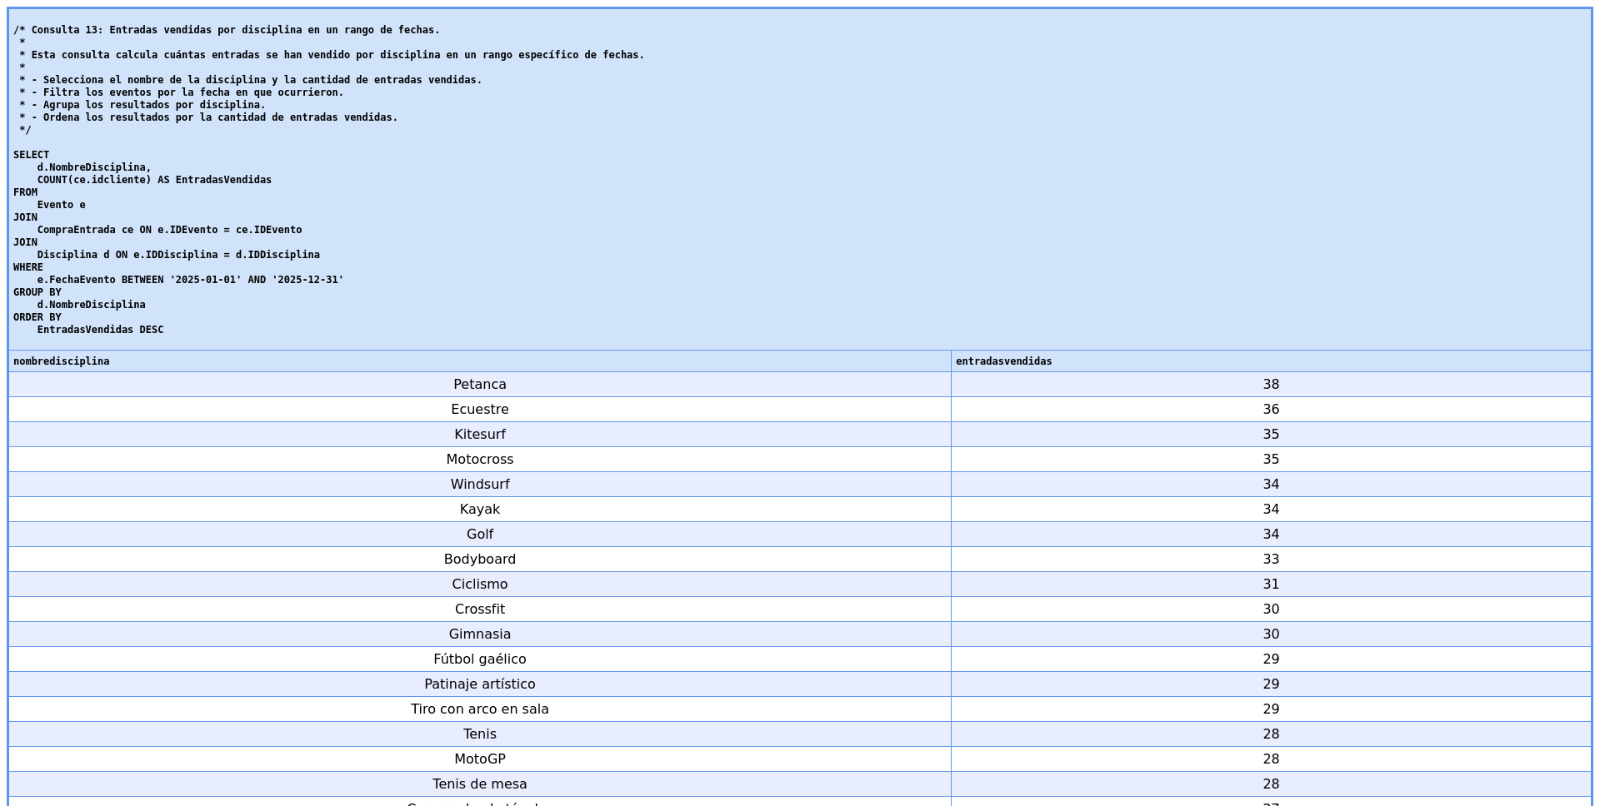
\includegraphics[width=16.5cm]{resources/Consulta13.jpeg} 
    
   Consulta 13. Entradas vendidas por disciplina en un rango de fechas.
\end{center}

\textbf{Propósito de la consulta}

El objetivo de esta consulta es determinar la cantidad de entradas vendidas por disciplina durante un rango específico de fechas. Esto permite analizar la popularidad de las disciplinas y apoyar la toma de decisiones en la planificación de futuros eventos.

\textbf{Desglose de la consulta}

\begin{itemize}
   \item \textbf{Selección de columnas (\texttt{SELECT})}:
   \begin{itemize}
       \item \texttt{d.NombreDisciplina}: Nombre de la disciplina deportiva.
       \item \texttt{COUNT(ce.IDCliente)}: Calcula la cantidad de entradas vendidas para cada disciplina. Esta columna se denomina \texttt{EntradasVendidas}.
   \end{itemize}

   \item \textbf{Tablas involucradas (\texttt{FROM} y \texttt{JOIN})}:
   \begin{itemize}
       \item \texttt{Evento (e)}: Contiene información sobre los eventos deportivos.
       \item \texttt{CompraEntrada (ce)}: Contiene información sobre las compras de entradas.
       \item \texttt{Disciplina (d)}: Contiene información sobre las disciplinas deportivas.
       \item Se realizan los siguientes \texttt{JOINs}:
       \begin{itemize}
           \item \texttt{Evento} con \texttt{CompraEntrada} usando \texttt{e.IDEvento = ce.IDEvento}, para relacionar las entradas con los eventos.
           \item \texttt{Evento} con \texttt{Disciplina} usando \texttt{e.IDDisciplina = d.IDDisciplina}, para asociar los eventos con las disciplinas correspondientes.
       \end{itemize}
   \end{itemize}

   \item \textbf{Filtrado de datos (\texttt{WHERE})}:
   \begin{itemize}
       \item Se filtran los eventos cuya fecha (\texttt{e.FechaEvento}) esté dentro del rango especificado: entre el 1 de enero y el 31 de diciembre de 2025.
   \end{itemize}

   \item \textbf{Agrupación de resultados (\texttt{GROUP BY})}:
   \begin{itemize}
       \item Los resultados se agrupan por \texttt{d.NombreDisciplina}, para calcular la cantidad total de entradas vendidas por cada disciplina.
   \end{itemize}

   \item \textbf{Ordenamiento de resultados (\texttt{ORDER BY})}:
   \begin{itemize}
       \item Los resultados se ordenan en orden descendente (\texttt{DESC}) según la cantidad de entradas vendidas (\texttt{EntradasVendidas}), mostrando primero las disciplinas más populares.
   \end{itemize}
\end{itemize}

\textbf{Análisis detallado}

\begin{enumerate}
   \item \textbf{Relación entre tablas:}
   \begin{itemize}
       \item Existe una relación entre las tablas \texttt{Evento}, \texttt{CompraEntrada} y \texttt{Disciplina}:
       \begin{itemize}
           \item Cada entrada comprada se asocia con un evento a través de \texttt{IDEvento}.
           \item Cada evento está vinculado a una disciplina mediante \texttt{IDDisciplina}.
       \end{itemize}
   \end{itemize}
   
   \item \textbf{Cálculo de entradas vendidas:}
   \begin{itemize}
       \item La función agregada \texttt{COUNT(ce.IDCliente)} cuenta el número de entradas vendidas asociadas con cada disciplina.
   \end{itemize}
   
   \item \textbf{Filtrado por rango de fechas:}
   \begin{itemize}
       \item El filtro en el \texttt{WHERE} asegura que solo se incluyan eventos ocurridos en 2025, excluyendo datos fuera de este rango temporal.
   \end{itemize}
   
   \item \textbf{Ordenamiento:}
   \begin{itemize}
       \item Ordenar por \texttt{EntradasVendidas DESC} permite identificar las disciplinas con mayor éxito en ventas de entradas.
   \end{itemize}
\end{enumerate}

\textbf{Consideraciones}

\begin{itemize}
   \item \textbf{Eventos sin ventas:}
   \begin{itemize}
       \item Si una disciplina no tuvo ventas de entradas, no aparecerá en los resultados.
   \end{itemize}
   \item \textbf{Empates en las ventas:}
   \begin{itemize}
       \item Si dos disciplinas tienen la misma cantidad de entradas vendidas, el orden relativo entre ellas no está definido. Se podría agregar un criterio adicional en el \texttt{ORDER BY}, como el nombre de la disciplina.
   \end{itemize}
\end{itemize}

\textbf{Utilidad de la consulta}

Esta consulta es útil para:
\begin{itemize}
    \item Evaluar la popularidad de las disciplinas en función de las ventas de entradas.
    \item Identificar disciplinas que podrían necesitar estrategias de promoción o mejor planificación logística.
    \item Ayudar en la asignación de recursos y espacios para futuras competencias basadas en la demanda histórica.
    \item Determinar patrones de participación del público durante un rango de fechas específico.
\end{itemize}

    \item \textbf{Consulta 14:} \begin{center}
    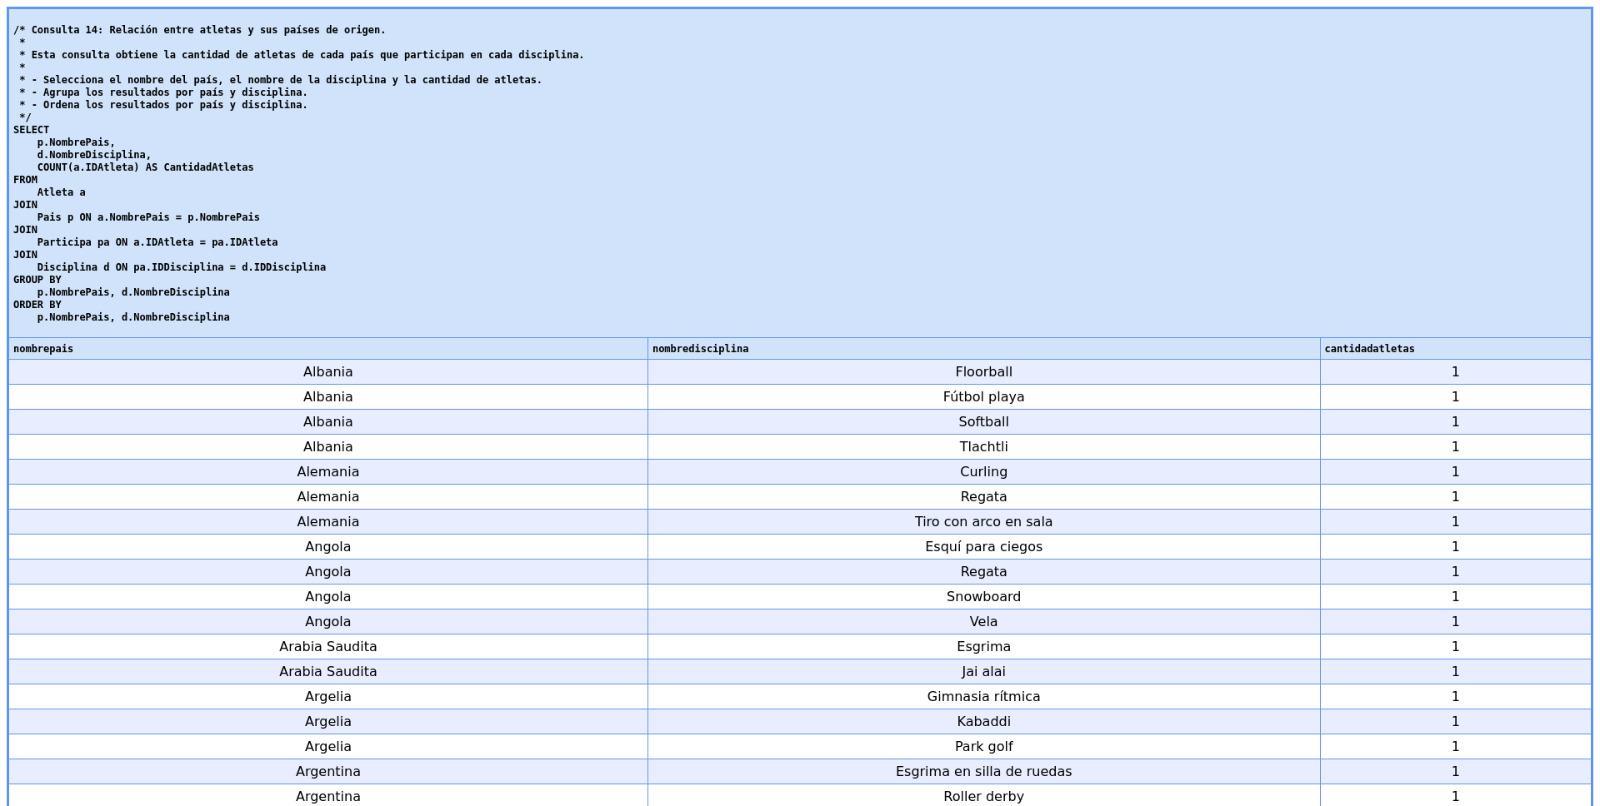
\includegraphics[width=16.5cm]{resources/Consulta14.jpeg} 
    
   Consulta 14. Relación entre atletas y sus países de origen.
\end{center}

\textbf{Propósito de la consulta}

El objetivo de esta consulta es obtener la cantidad de atletas de cada país que participan en cada disciplina. Esto permite analizar la representación de los países en diferentes disciplinas y evaluar la diversidad en las competencias deportivas.

\textbf{Desglose de la consulta}

\begin{itemize}
   \item \textbf{Selección de columnas (\texttt{SELECT})}:
   \begin{itemize}
       \item \texttt{p.NombrePais}: Nombre del país de origen de los atletas.
       \item \texttt{d.NombreDisciplina}: Nombre de la disciplina deportiva.
       \item \texttt{COUNT(a.IDAtleta)}: Calcula la cantidad de atletas por país en cada disciplina, generando la columna \texttt{CantidadAtletas}.
   \end{itemize}

   \item \textbf{Tablas involucradas (\texttt{FROM} y \texttt{JOIN})}:
   \begin{itemize}
       \item \texttt{Atleta (a)}: Contiene información sobre los atletas.
       \item \texttt{Pais (p)}: Contiene información sobre los países de origen.
       \item \texttt{Participa (pa)}: Relaciona a los atletas con las disciplinas en las que participan.
       \item \texttt{Disciplina (d)}: Contiene información sobre las disciplinas deportivas.
       \item Se realizan los siguientes \texttt{JOINs}:
       \begin{itemize}
           \item \texttt{Atleta} con \texttt{Pais} usando \texttt{a.NombrePais = p.NombrePais}, para asociar a cada atleta con su país de origen.
           \item \texttt{Atleta} con \texttt{Participa} usando \texttt{a.IDAtleta = pa.IDAtleta}, para identificar las disciplinas en las que participa cada atleta.
           \item \texttt{Participa} con \texttt{Disciplina} usando \texttt{pa.IDDisciplina = d.IDDisciplina}, para relacionar cada participación con una disciplina específica.
       \end{itemize}
   \end{itemize}

   \item \textbf{Agrupación de resultados (\texttt{GROUP BY})}:
   \begin{itemize}
       \item Los resultados se agrupan por \texttt{p.NombrePais} y \texttt{d.NombreDisciplina}, para calcular la cantidad de atletas por país en cada disciplina.
   \end{itemize}

   \item \textbf{Ordenamiento de resultados (\texttt{ORDER BY})}:
   \begin{itemize}
       \item Los resultados se ordenan primero por \texttt{p.NombrePais} (nombre del país) y luego por \texttt{d.NombreDisciplina} (nombre de la disciplina), facilitando la lectura y análisis.
   \end{itemize}
\end{itemize}

\textbf{Análisis detallado}

\begin{enumerate}
   \item \textbf{Relación entre tablas:}
   \begin{itemize}
       \item La consulta establece relaciones entre las tablas \texttt{Atleta}, \texttt{Pais}, \texttt{Participa} y \texttt{Disciplina}, conectando a cada atleta con su país y las disciplinas en las que participa.
   \end{itemize}
   
   \item \textbf{Cálculo de atletas:}
   \begin{itemize}
       \item La función agregada \texttt{COUNT(a.IDAtleta)} cuenta el número de atletas de un país que participan en cada disciplina.
   \end{itemize}
   
   \item \textbf{Agrupación:}
   \begin{itemize}
       \item El \texttt{GROUP BY} asegura que los datos estén organizados de manera que cada combinación de país y disciplina tenga su correspondiente conteo.
   \end{itemize}
   
   \item \textbf{Ordenamiento:}
   \begin{itemize}
       \item El orden jerárquico por país y disciplina facilita la interpretación, permitiendo identificar rápidamente la representación por país en cada deporte.
   \end{itemize}
\end{enumerate}

\textbf{Consideraciones}

\begin{itemize}
   \item \textbf{Atletas sin participación:}
   \begin{itemize}
       \item Si un atleta no está asociado a una disciplina, no aparecerá en los resultados.
   \end{itemize}
   \item \textbf{Empates en cantidad de atletas:}
   \begin{itemize}
       \item Si dos países tienen la misma cantidad de atletas en una disciplina, el orden entre ellos no está definido. Se podría agregar un criterio adicional en el \texttt{ORDER BY}, como el nombre del país o de la disciplina.
   \end{itemize}
\end{itemize}

\textbf{Utilidad de la consulta}

Esta consulta es útil para:
\begin{itemize}
    \item Analizar la diversidad de participación en cada disciplina y verificar la representación equitativa de diferentes países.
    \item Identificar posibles tendencias en la participación de atletas de determinados países en disciplinas específicas.
    \item Planificar estrategias de inclusión y promoción para fomentar la participación de países con poca representación.
    \item Facilitar reportes y estadísticas sobre la participación internacional en competencias deportivas.
\end{itemize}

    \item \textbf{Consulta 15:} \begin{center}
    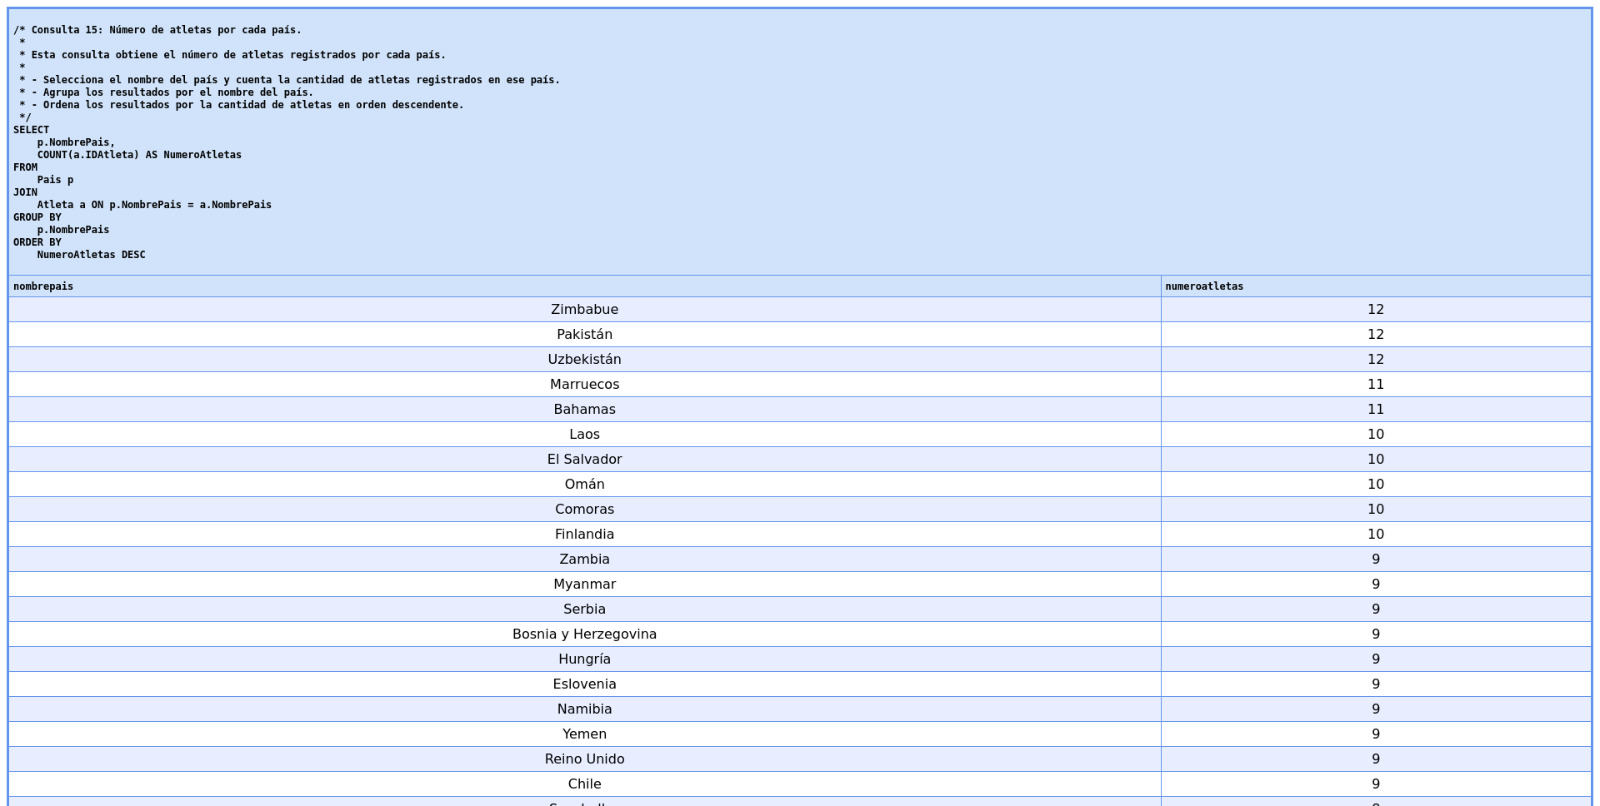
\includegraphics[width=16.5cm]{resources/Consulta15.jpeg} 
    
   Consulta 15. Número de atletas por cada país.
\end{center}

\textbf{Propósito de la consulta}

El objetivo de esta consulta es determinar cuántos atletas están registrados en cada país, proporcionando una visión general de la distribución de atletas a nivel internacional.

\textbf{Desglose de la consulta}

\begin{itemize}
   \item \textbf{Selección de columnas (\texttt{SELECT})}:
   \begin{itemize}
       \item \texttt{p.NombrePais}: Nombre del país de origen de los atletas.
       \item \texttt{COUNT(a.IDAtleta)}: Calcula el número total de atletas registrados en cada país. Esta columna se denomina \texttt{NumeroAtletas}.
   \end{itemize}

   \item \textbf{Tablas involucradas (\texttt{FROM} y \texttt{JOIN})}:
   \begin{itemize}
       \item \texttt{Pais (p)}: Contiene información sobre los países.
       \item \texttt{Atleta (a)}: Contiene información sobre los atletas.
       \item Se realiza un \texttt{JOIN} entre \texttt{Pais} y \texttt{Atleta} utilizando la relación \texttt{p.NombrePais = a.NombrePais}, que vincula a cada atleta con su país de origen.
   \end{itemize}

   \item \textbf{Agrupación de resultados (\texttt{GROUP BY})}:
   \begin{itemize}
       \item Los resultados se agrupan por \texttt{p.NombrePais}, para calcular el número de atletas registrados en cada país.
   \end{itemize}

   \item \textbf{Ordenamiento de resultados (\texttt{ORDER BY})}:
   \begin{itemize}
       \item Los resultados se ordenan en orden descendente (\texttt{DESC}) según la cantidad de atletas (\texttt{NumeroAtletas}), mostrando primero los países con más atletas registrados.
   \end{itemize}
\end{itemize}

\textbf{Análisis detallado}

\begin{enumerate}
   \item \textbf{Relación entre tablas:}
   \begin{itemize}
       \item La consulta utiliza la relación entre las tablas \texttt{Pais} y \texttt{Atleta} para asociar a cada atleta con su país de origen.
   \end{itemize}
   
   \item \textbf{Cálculo de atletas:}
   \begin{itemize}
       \item La función agregada \texttt{COUNT(a.IDAtleta)} cuenta el número de atletas registrados en cada país.
   \end{itemize}
   
   \item \textbf{Agrupación:}
   \begin{itemize}
       \item El uso de \texttt{GROUP BY} organiza los resultados por país, asegurando que cada país tenga un registro único con su conteo correspondiente de atletas.
   \end{itemize}
   
   \item \textbf{Ordenamiento:}
   \begin{itemize}
       \item El orden descendente por \texttt{NumeroAtletas} facilita la identificación de los países con mayor cantidad de atletas registrados.
   \end{itemize}
\end{enumerate}

\textbf{Consideraciones}

\begin{itemize}
   \item \textbf{Países sin atletas registrados:}
   \begin{itemize}
       \item Los países que no tienen atletas registrados no aparecerán en los resultados.
   \end{itemize}
   \item \textbf{Empates en cantidad de atletas:}
   \begin{itemize}
       \item Si dos o más países tienen el mismo número de atletas registrados, el orden relativo entre ellos no está definido. Se podría agregar un criterio adicional en el \texttt{ORDER BY}, como el nombre del país.
   \end{itemize}
\end{itemize}

\textbf{Utilidad de la consulta}

Esta consulta es útil para:
\begin{itemize}
    \item Analizar la distribución de atletas a nivel internacional.
    \item Identificar países con una alta o baja representación en términos de atletas registrados.
    \item Planificar estrategias para fomentar la participación en países con menor número de atletas.
    \item Evaluar la diversidad y alcance global del registro de atletas.
\end{itemize}

    \item \textbf{Consulta Extra:} \begin{center}
    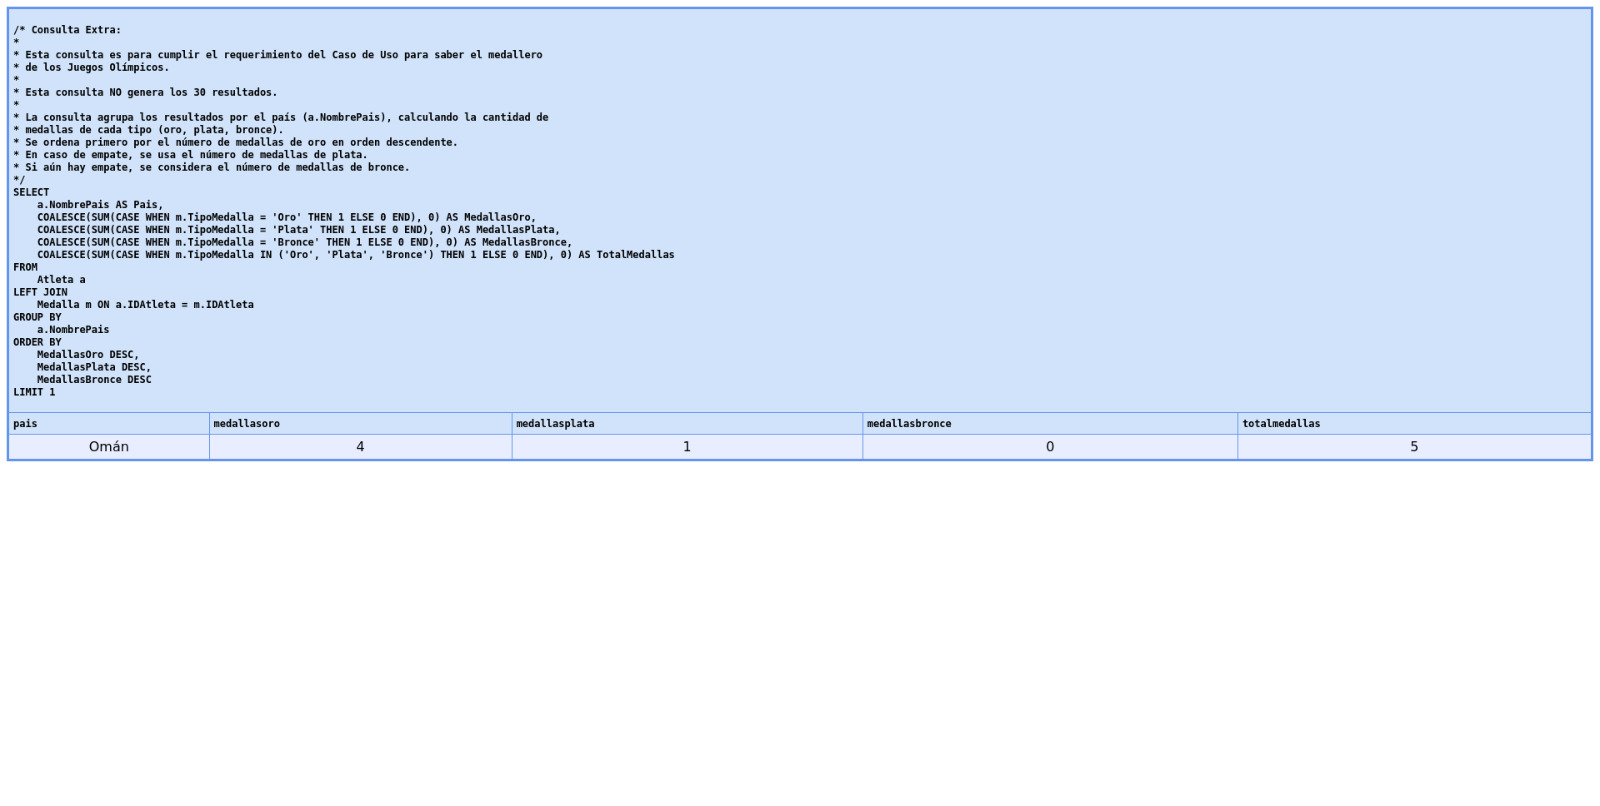
\includegraphics[width=16.5cm]{resources/ConsultaExtra.jpeg} 
    
   Consulta Extra. Medallero de los Juegos Olímpicos.
\end{center}

\textbf{Propósito de la consulta}

El objetivo de esta consulta es generar el medallero de los Juegos Olímpicos, mostrando la cantidad de medallas de oro, plata y bronce obtenidas por cada país, con un orden que prioriza el número de medallas de oro, seguido por las de plata y bronce.

\textbf{Desglose de la consulta}

\begin{itemize}
   \item \textbf{Selección de columnas (\texttt{SELECT})}:
   \begin{itemize}
       \item \texttt{a.NombrePais}: Nombre del país que será representado en el medallero.
       \item \texttt{COALESCE(SUM(CASE ...))}: Suma la cantidad de medallas de cada tipo (oro, plata, bronce), reemplazando valores nulos con 0.
       \item \texttt{TotalMedallas}: Suma total de medallas (oro, plata y bronce) obtenidas por el país.
   \end{itemize}

   \item \textbf{Tablas involucradas (\texttt{FROM} y \texttt{JOIN})}:
   \begin{itemize}
       \item \texttt{Atleta (a)}: Contiene información sobre los atletas y su país de origen.
       \item \texttt{Medalla (m)}: Contiene información sobre las medallas obtenidas por los atletas.
       \item Se utiliza un \texttt{LEFT JOIN} entre \texttt{Atleta} y \texttt{Medalla} para incluir a los países incluso si no tienen medallas registradas.
   \end{itemize}

   \item \textbf{Agrupación de resultados (\texttt{GROUP BY})}:
   \begin{itemize}
       \item Los resultados se agrupan por \texttt{a.NombrePais}, asegurando que cada país tenga un único registro con el conteo de sus medallas.
   \end{itemize}

   \item \textbf{Ordenamiento de resultados (\texttt{ORDER BY})}:
   \begin{itemize}
       \item Los resultados se ordenan jerárquicamente:
       \begin{enumerate}
           \item Por \texttt{MedallasOro} en orden descendente.
           \item En caso de empate, por \texttt{MedallasPlata}.
           \item En caso de persistir el empate, por \texttt{MedallasBronce}.
       \end{enumerate}
   \end{itemize}

   \item \textbf{Límite de resultados (\texttt{LIMIT 1})}:
   \begin{itemize}
       \item La consulta devuelve solo el país con más medallas de oro (y desempates por plata y bronce), ya que está limitada a un solo resultado.
   \end{itemize}
\end{itemize}

\textbf{Análisis detallado}

\begin{enumerate}
   \item \textbf{Relación entre tablas:}
   \begin{itemize}
       \item La consulta vincula a los atletas con las medallas que han ganado utilizando \texttt{a.IDAtleta = m.IDAtleta}.
       \item El \texttt{LEFT JOIN} asegura que los países sin medallas aún se incluyan en la lista, aunque con valores de medallas igual a cero.
   \end{itemize}

   \item \textbf{Cálculo de medallas:}
   \begin{itemize}
       \item Las expresiones \texttt{CASE WHEN} cuentan medallas específicas (oro, plata, bronce), sumando los valores que corresponden.
       \item \texttt{COALESCE} reemplaza valores nulos con 0, útil para países que no tienen medallas de cierto tipo.
   \end{itemize}

   \item \textbf{Orden y desempate:}
   \begin{itemize}
       \item El orden por tipos de medallas asegura que los países con mejor desempeño sean priorizados correctamente.
   \end{itemize}
\end{enumerate}

\textbf{Consideraciones}

\begin{itemize}
   \item \textbf{Países sin medallas:}
   \begin{itemize}
       \item Gracias al \texttt{LEFT JOIN}, los países sin medallas no son excluidos, pero tendrán valores de medallas igual a cero.
   \end{itemize}
   \item \textbf{Empates:}
   \begin{itemize}
       \item Si dos países tienen exactamente el mismo número de medallas de oro, plata y bronce, el orden relativo entre ellos no está definido.
   \end{itemize}
\end{itemize}

\textbf{Utilidad de la consulta}

Esta consulta permite:
\begin{itemize}
    \item Generar estadísticas sobre el rendimiento de cada país en los Juegos Olímpicos.
    \item Identificar rápidamente el país más exitoso basado en el conteo de medallas.
    \item Evaluar tendencias en el desempeño de países durante la competencia.
\end{itemize}

\textbf{Nota sobre el \texttt{LIMIT 1}}

Si se elimina la cláusula \texttt{LIMIT 1}, la consulta generará el medallero completo, mostrando los resultados para todos los países en orden de prioridad basado en el número de medallas de oro, plata y bronce.

\end{itemize}